%
% Idee zum Projekt
%
\chapter{Projektidee und Analyse}
\label{cap-projektidee}

\section{Hintergrund: Praxisphase eines Bachelor Studenten Angewandte Informatik}
\label{sec-idee-hintergrund}

Der Bachelor Studiengang Angewandte Informatik (AI) an der Hochschule Ravensburg-Weingarten ist auf 6 Semester ausgelegt. Dies wird dadurch möglich, dass die Studenten in ihrem 6. Semester neben 3 Monaten Praxisphase die übrigen 3 Monate zum Schreiben ihrer Bachelorarbeit nutzen müssen. Viele Studenten gehen daher nach der von der Hochschule empfohlenen Methode vor und absolvieren beides bei einer Firma. Das verringert die Einarbeitungszeit und ermöglicht es, schnell ein Thema für die Bachelor Arbeit zu finden. Dadurch gewinnt die Auswahl einer passenden Firma an Bedeutung.

Die Hochschule versucht schon frühzeitig Firmen und Studenten durch Veranstaltungen wie den Karrieretagen zusammenzubringen. Trotzdem stehen die Studenten am Anfang ihres 5. Semesters vor der Aufgabe jetzt möglichst schnell eine Firma zu finden. 

\paragraph{Schwerpunkte}
Dabei ist es nicht möglich bei jeglichen Firmen zu arbeiten. Die Aufgaben in der Firma müssen weitestgehend mit dem gelernten Wissen in den Schwerpunkten übereinstimmen. Die Schwerpunkte werden von den Studenten bereits im 3. Semester gewählt. Dabei müssen zwei aus drei zur Zeit möglichen Schwerpunkten ausgewählt werden. Daher muss der Student nicht nur eine Firma finden, die seine eigenen Interessen möglichst gut abbildet, sondern es sollten auch die gewählten Schwerpunkte berücksichtigt sein.

\paragraph{Firmenbewertungen}
Nach Abschluss der Praxisphase werden die Firmen nach einigen, vom Leiter des Praktikantenamts vorgegebenen, Kriterien bewertet. Diese Bewertungen finden seit einiger Zeit online mit dem Umfragetool \gls{INKIDU}\footnote{\url{http://www.inkidu.hs-weingarten.de}} statt.

\paragraph{Professoren}
Sowohl für die Praxisphase als auch für eine Bachelor-Arbeit benötigen die Studenten einen betreuenden Professor, welche als Dozenten bei bei bestimmten Veranstaltungen auftreten.

\section{Idee: Automatische Empfehlung einer Firma}
\label{sec-idee-projekt}
\paragraph{Grundidee} Der Student soll, basierend auf den \textbf{Veranstaltungen} (z. B. Vorlesungen) die er im Rahmen seines gewählten \textbf{Schwerpunkts} besucht hat, eine Liste der Firmen erhalten, die am Besten zu diesen Veranstaltungen passen. Optional soll der Student seine Interessen angeben können, welche ebenfalls bei der Empfehlung berücksichtigt werden.

Welche Firma gut zu den gewählten Schwerpunkten und den Präferenzen des Studenten passt, wird anhand der Bewertungen aus vorherigen Praxisphasen ermittelt. Welcher Professor gut zu einer gewählten Firma passt, soll anhand der Veranstaltungen bei denen ein Professor Dozent ist entschieden werden.

Zu beiden Empfehlungen, Firma und Professor, soll es jeweils auch Alternativen geben, also das Ergebnis dieser Klassifizierung (siehe \ref{klassifizierung}) soll eine sortierte Liste sein. Bei der die Firma, die am besten ``passt'', als erstes genannt ist. Zu jeder Firma soll eine sortierte Liste mit Professoren angegeben werden.

\section{Analyse: Datenformate und Vorgehensweise} % war: Analyse der Projektidee
\label{sec-analyse-daten}
Nachdem die Grundidee skizziert ist, stellt sich die Frage woher die Daten kommen, um eine solche Anwendung zu bauen. Aber nicht nur die Quelle der Daten ist wichtig, auch deren Format für die Weiterverarbeitung. Genau zu dieser Fragestellung wollen wir hier eine Antwort finden.

\subsection{Warum Ontologien/Linked Data/Semantic Web nutzen?}
Der klassische Ansatz für ein Problem, wie das im vorherigen Abschnitt beschriebene, ist eine Anwendung mit einer relationalen Datenbank. Hier können die ganzen Daten aus den Quellen gesammelt werden und mit SQL und etwas ``Geschäfts-Logik'' kann die Anwendung einfach realisiert werden.

Warum sollte man sich also die Mühe machen und sperrige XML basierte Dokumente erstellen wie RDF? Wieso sollte man neue Abfragesprechen wie SPARQL lernen? Der Nutzen im Verhältnis zum Aufwand, wird bei der Betrachtung  \textit{einer Anwendung} nicht direkt deutlich.

Macht man sich aber klar, dass die Daten auch für andere Anwendungen von Bedeutung sein könnten dann wird schnell klar, dass es doch Sinn macht diese Daten in den vom W3C empfohlenen Sprachen zu beschreiben. Problematisch ist dieser Ansatz weil Unternehmen und Behörden so nicht denken. Erst wenn es einen Bedarf an Daten von externer Seite gibt, wird eine, meist spezifische, Schnittstelle geschaffen.

\subsection{Open Linked-Data an der HS Weingarten}
\label{sec-open-linked-data-hs}
Im Idealfall wären alle Daten schon öffentlich in einem Standardformat zugänglich. Es fehlt also zunächst eine API für Daten der einzelnen Dienste an der Hochschule. Ideal wäre es, wenn die Dienste die Daten als Linked-Data veröffentlichen würden. Dies würde es ermöglichen, die Daten aus den verschiedenen Quellen (Hochschulintern sowie mit externen Quellen; siehe dazu \ref{sec-dathubs}) direkt zu kombinieren.

Das Semantic Web kann nur dann eine Bedeutung erlangen, wenn Webangebote, wie das unserer Hochschule, anfangen die Daten auch semantisch zur Verfügung zu stellen. Bisher gibt es von offizieller Stelle dazu keine Planungen. Daher ist eines unserer Ziele in diesem Projekt: 
\begin{quote}
\textbf{Öffentliche Daten der Hochschule semantisch aufzubereiten und zur Verfügung zu stellen}.
\end{quote}

\subsection{Datenquellen}
\label{sec-idee-datenquellen}
\begin{figure}[h]
	\centering
	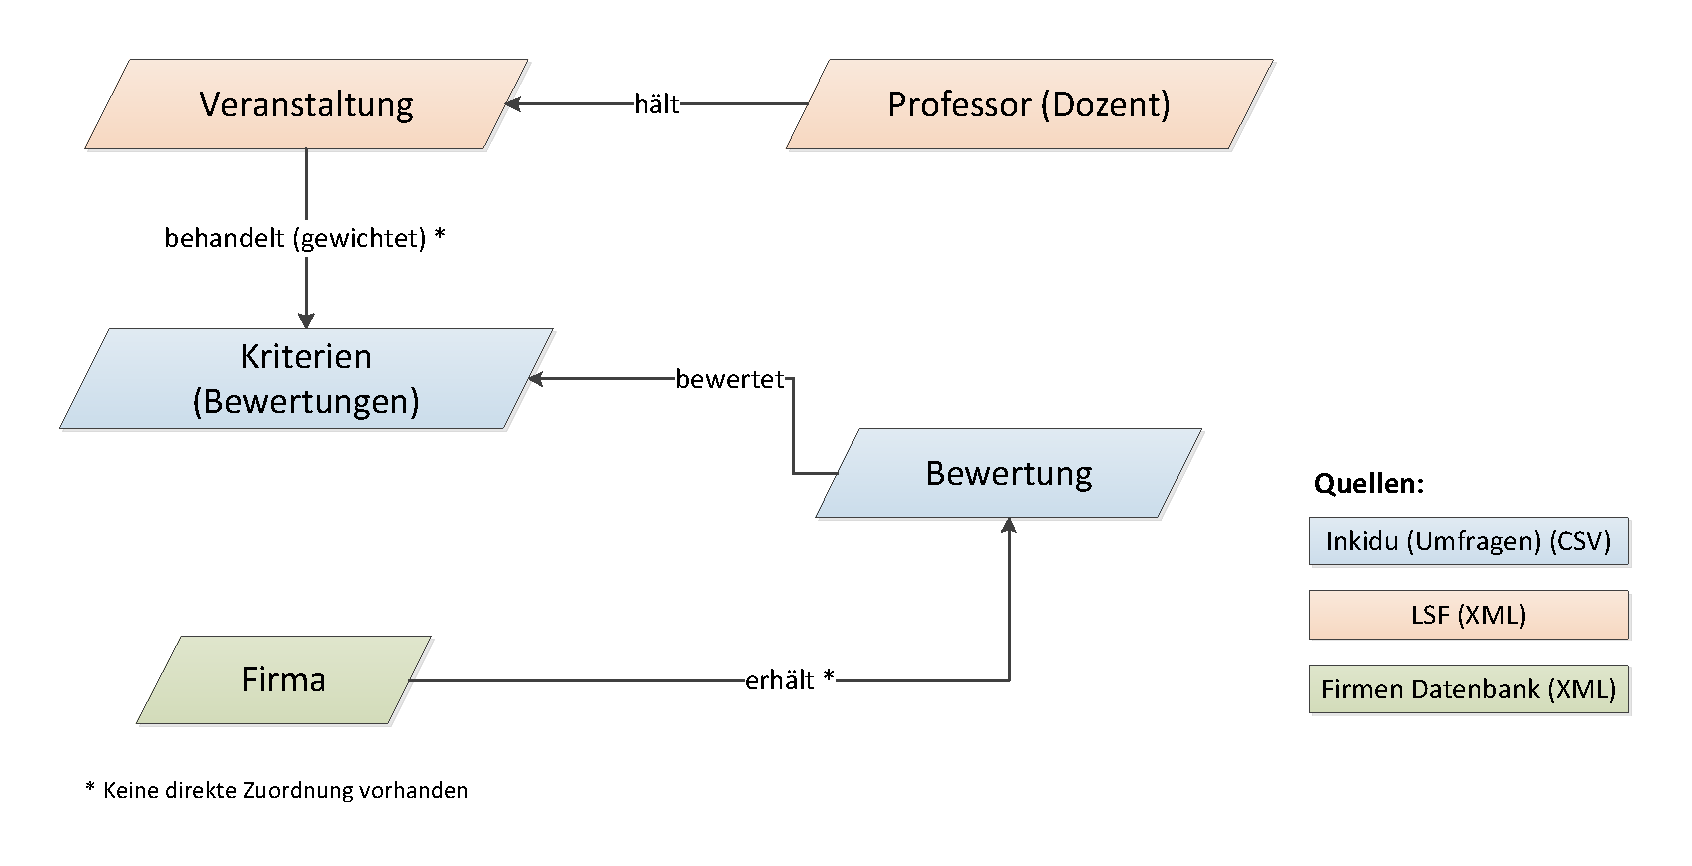
\includegraphics[scale=0.53]{images/Highlevel-Daten-Verkuepfung-Herkunft}
	\caption{Benötigte Daten und deren Beziehungen (vereinfacht)}
	\label{graphic-highlevel-data}
\end{figure}

Abbildung \ref{graphic-highlevel-data} zeigt die Daten und deren Beziehungen. In dieser stark vereinfachten Darstellung kann man die Zusammenhänge zwischen den Daten leicht erkennen. Auch deren Quellen, sowie das Format wird in der Grafik kurz angedeutet.

%\subsection{Datenquellen} %\subsection{Open Linked Data an der Hochschule}
Die Daten an der Hochschule über Veranstaltungen oder Professoren werden im sogenannten \gls{LSF} der Firma HIS verwaltet. Dabei werden einige Informationen auch öffentlich als HTML ausgeliefert. Leider werden diese Informationen nicht als Triples (z.B. in RDF) veröffentlicht. Es gibt lediglich auf Anfrage beim Rechenzentrum eine XML Schnittstelle bei der die benötigten Daten aus der Datenbank verfügbar gemacht werden können.


%\subsubsection{Formate und Konvertierung} % überflüssig???
Wie in Abbildung \ref{graphic-highlevel-data} bereits unter Quellen zu sehen, gibt es 3 primäre Datenquellen für unsere Anwendung an der Hochschule. Die mit * gekennzeichneten Verbindungen sind nicht vorhanden bzw. lassen sich nicht direkt aus den Daten ableiten.

\paragraph{LSF} Das LSF\footnote{\url{http://www.lsf.hs-weingarten.de}} bietet einen XML Export. Leider ist diese Schnittstelle noch nicht so weit ausgebaut als das wir sie für unser Projekt nutzen könnten. Daher wurden die LSF Daten exemplarisch von Hand ermittelt. Verbindungen zwischen Veranstaltung und Dozenten (Professoren) sind jedoch eindeutig.

\paragraph{Fimen Datenbank} Die Firmendatenbank (PDB) wird von Hand von der LeiterIn des Praktikantenamts gepflegt. Manuell werden die Daten als XML auf einem Webserver abgelegt.

\paragraph{INKIDU} Das Online Umfragesystem INKIDU\footnote{\url{http://inkidu.de}} ermöglicht einen \gls{CSV} Export der Umfrageergebnisse. Dieses System erlaubt dem Nutzer nur Freitextfelder und bietet daher keine Verbindung zwischen den Umfrageergebnissen und den Daten die zu einer Firma in der Firmendatenbank gespeichert sind. Ideen für die Zuordnung finden sich im Abschnitt \ref{sec-algo}.


\subsection{Algorithmen}
\label{sec-algo}
Um aus den Daten ``Linked Data'' zu machen, können verschiedene Techniken angewandt werden. Primär geht es darum, eine Zuordnung zwischen nicht direkt verbundenen Datensätzen zu finden. Ein weiterer Aspekt bei der Veröffentlichung von Daten ist der Datenschutz. Da es sich bei den Bewertungen um Meinungen von Studenten über Firmen handelt, dürfen diese natürlich nicht direkt veröffentlicht werden.

\subsubsection{Firmenzuordnung} % andreas
Wie bereits mehrfach erwähnt, gibt es keine Zuordnung zwischen den Firmen in der Firmen Datenbank und den Bewertungen der Studenten. Dadurch, dass die Daten in verschiedensten Formaten vorliegen und auch nicht in einem einheitlichen Konzept abgelegt wurden, bzw. keine eindeutige Identität haben, ist es nur möglich diese anhand eines Pattern-Matching-Verfahrens zu vergleichen und die größtmögliche Ähnlichkeit als Referenz zu verwenden.\\
Dabei wird ein String, der einen Firmennamen repräsentiert, anhand der im String vorkommenden einzelnen Worte unterteilt und dabei ausgehend von rechts nach links mit dem vorliegenden String verglichen. Wichtig ist dabei, dass unbedingt von rechts angefangen werden muss den String zu vergleichen, da in der deutschen Sprache Firmennamen immer mit der Gesellschaftsform am Ende definiert werden.
Nehmen wir einmal das Beispiel
\begin{verbatim}
 Mayer Informatik GmbH
\end{verbatim}
so würde dies maximal drei Durchläufe zum Vergleich ergeben:
\begin{verbatim}
 Mayer Informatik GmbH
 Mayer Informatik
 Mayer
\end{verbatim}
Dabei kann es natürlich passieren, dass zum Ergebnis \texttt{Mayer} mehrere Einträge in der Firmendatenbank gefunden werden, aber dies ist anhand der vorliegenden Daten leider nicht zu vermeiden. Ist nach dem dritten Durchlauf immer noch kein Matching möglich, so wird der Versuch erfolglos abgebrochen. In beiden Fällen wird die Firma im Ergebnis nicht angezeigt.

\subsubsection{Bayesian average}
Der CSV Export der INKIDU Umfragen enthält jede Firmenbewertung einzeln.
Aus Datenschutzgründen müssen diese Bewertungen vor der Veröffentlichung auf einen Wert pro Firma aggregiert werden.
Um eine faire Gewichtung zwischen Firmen mit vielen Bewertungen und welchen mit wenigen zu erreichen wird die ``Bayesian average'' (\ref{eq:bayesavg}) berechnet.

\begin{equation}
\bar{x} = {Cm + \sum_{i=1}^n{x_i} \over C + n} 	\label{eq:bayesavg}
\end{equation}

Hierbei ist $C$ die durchschnittliche Anzahl der Bewertungen, $m$ der A-priori Durchschnitt und $n$ die Anzahl der Bewertungen für dieses Element.
Eine praktische Erklärung ist in \cite{Weichs06} zu finden.

% Hier Nur Algos für die Datenkonvertierung KEINE für die eigentlich Anwendung!!!

\section{Datenmodellierung im Projekt} 	% war: Design des Projekts
\label{sec-idee-datenmodel}
\subsection{Ontologien}
Ziel beim Aufbau der Ontologie für unseren Anwendungsfall ist es, so viele standardisierte ``Terms'' zu verwenden wie möglich. Sich also stets bei anderen, bekannten und etablierten Ontologien zu bedienen.
Es soll nachher keine völlig neue Ontologie entstehen, sondern nur die Teile für die es keine ``Terms'' gibt erweitert werden. Im Sinne des Semantic Web Gedanken, sollten Daten wie Bezeichnungen von Objekten möglichst mit den bekannten Terms bezeichnet werden. 

In dem Vortrag von Tim Berners Lee vom Mai 2010  \cite{W3CQALD} greift er die Problematik der Zurückhaltung vieler Entwickler in Sachen Semantic Web auf. Viele Entwickler haben das Semantic Web missverstanden, prangert der Web-Erfinder an und versucht es anhand einer Tüte Kartoffelchips für jeden verständlich zu erklären. Es wird keine große universalgültige Ontologie geben, doch das darf uns nicht davon abhalten die Techniken nicht einzusetzen. \textit{Open Your Data NOW!}

Im Folgenden werden Ontologien, die wir im Projekt benutzt haben, vorgestellt:

\paragraph{DC}
Dublin Core\footnote{\url{http://dublincore.org}} beschreibt grundlegende Metadaten-Elemente. Die Elemente wie Titel, Ersteller, Thema, Beschreibung, Datum und Sprache sind allgemeingültig genug um viele Dinge wie Bücher, Filme, Bilder oder Web Seiten zu beschreiben.
Dublin Core ist auch als ISO Standard 15836 festgelegt.

\paragraph{FOAF}
\label{foaf}
Friend of a Friend\footnote{\url{http://www.foaf-project.org}} ermöglicht es Menschen und ihre Beziehungen untereinander maschinenlesbar darzustellen.
Dazu gehört zum einen Menschen zu beschreiben, also Eigenschaften wie Namen, Alter, Email Adresse und Website zu definieren.
Zum anderem werden Relationen zwischen Personen modelliert. Dies kann entweder über direkte ``knows'' Beziehung zwischen Menschen geschehen oder über Gruppenzugehörigkeiten.

Die Spezifikation\footnote{\url{http://xmlns.com/foaf/spec/}} wird stets weiterentwickelt und wurde zuletzt im Januar 2010 aktualisiert.
Viele soziale Netzwerke wie LiveJournal und identi.ca\footnote{\url{http://identi.ca}} bieten FOAF Informationen über ihre Nutzer an.
Daraus resultiert, dass FOAF einen Großteil der im Web verfügbaren semantischen Daten repräsentiert.
Auch in Zukunft wird FOAF eine wichtige Rolle spielen, wenn soziale Netzwerke via FOAF+SSL\footnote{\url{http://esw.w3.org/Foaf\%2Bssl}} oder mit Diaspora\footnote{\url{http://www.joindiaspora.com}} komplett dezentral werden.

\paragraph{AIISO}
Die \gls{AIISO}\footnote{\url{http://vocab.org/aiiso/schema}} ist eine Ontologie mit welcher die Struktur von akademischen Instituten beschrieben wird.
Es können Lehreinheiten wie Kurse, Fächer und Module beschrieben werden. Diese können, ganz im Sinne von Linked-Data, wiederum andere Lehreinheiten enthalten und auf diese verweisen.
Des weiteren können Fakultäten, Departments, Institute und ihre Zusammenhänge beschrieben werden.

\paragraph{SKOS}
\gls{SKOS}\footnote{\url{http://www.w3.org/2004/02/skos/}} ist ein einfaches \gls{KOS} für das Semantic Web.
Die vom W3C selbst entwickelte Spezifikation\footnote{\url{http://www.w3.org/TR/skos-reference/}} erlaubt es ein eigenes Vokabular zu veröffentlichten.
Somit ist es möglich Konzepte und Begriffe für ein Klassifizierungsschema oder eine Taxonomie zu definieren.

\paragraph{Eigene Definition}

\begin{figure}[htbp]
	\centering
	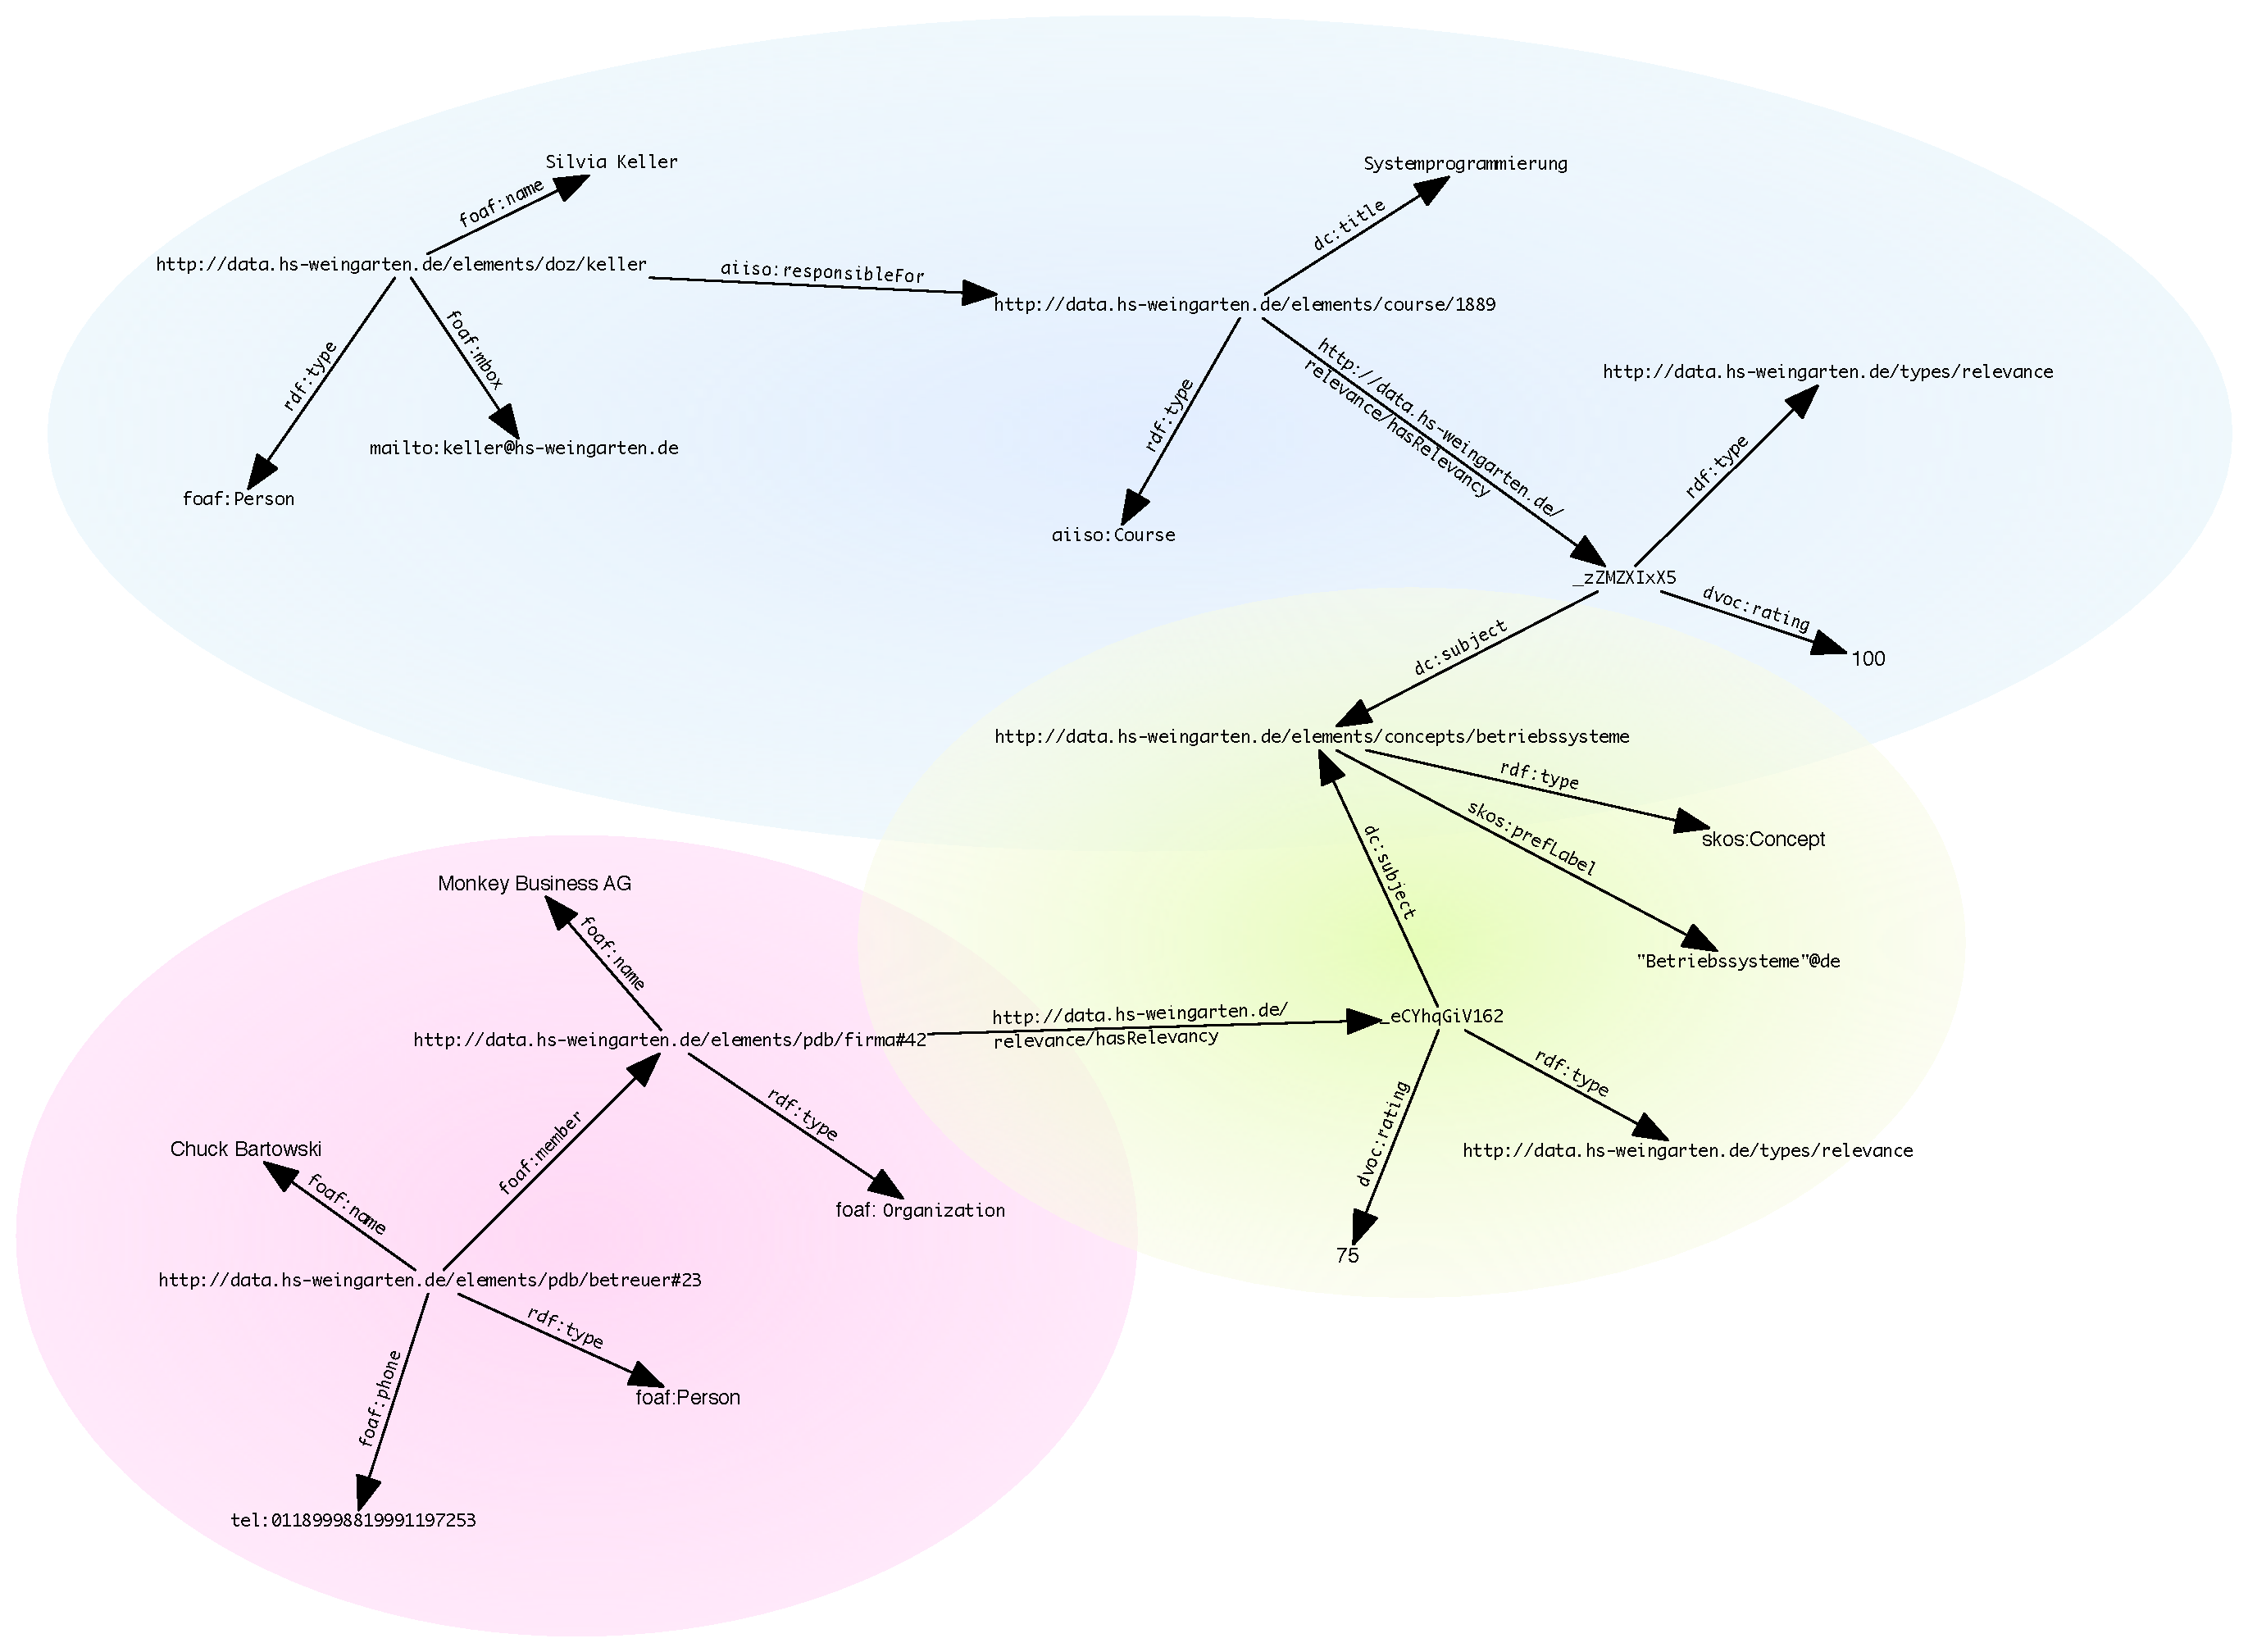
\includegraphics[scale=0.45,angle=90]{images/graph.pdf}
	\caption{Aufbau des Datenmodells an einem konkreten Beispiel}
	\label{example-graph}
\end{figure}

Ein Großteil der verwendeten Daten kann also mit bereits bestehenden Ontologien modelliert werden.
Einzig für die Relevanz-Information zwischen einem Topic (skos:Concept) und einem anderem Subjekt wurde ein eigenes Format definiert.
Die Zusammenhänge der Daten werden in Abbildung \ref{example-graph} verdeutlicht.

Es ist empfehlenswert bekannte und bereits bestehende Ontologien einzusetzen, da somit das Verbinden mehrerer Datenquellen vereinfacht wird.
Auch wenn dies keine harte Anforderung ist, da man mit ``owl:sameAs'' relativ einfach mappings zwischen unterschiedlichen Ontologien herstellen kann,
ist es dennoch sinnvoll auf bereits bestehenden Arbeiten aufzubauen.
Aus diesem Grund werden weitere Empfehlungen für Ontologien in \cite{ONTOPAT} aktiv mit der Community als Wiki diskutiert.
\newpage
\subsection{Daten veröffentlichen} 			% Data fetching / publishing
Die Daten werden als RDF Dateien auf einem Webserver abgelegt. Zusätzlich soll ein SPARQL Endpoint dafür sorgen, das jeder direkte Abfragen über Daten machen kann.

Die Subdomain ``data'' hat sich für die Veröffentlichung von (semantischen) Daten bewährt.
Prominente Beispiele:
\begin{itemize}
 \item \href{http://data.gov}{data.gov} - US Regierung
 \item \href{http://data.gov.uk}{data.gov.uk} - UK Regierung
 \item \href{http://data.worldbank.com}{data.worldbank.com} - Weltbank
 \item \href{http://data.nytimes.com}{data.nytimes.com} - New York Times
\end{itemize}

Daher wäre die Adresse \textbf{data.hs-weingarten.de} wünschenswert.

\section{Klassifizierung der Firmen und Professoren}		% Decision making by benny
\label{klassifizierung}
Sind alle Daten als ">Linked Data"< verfügbar, muss unsere Anwendung die Firmen und Professoren den gewählten Schwerpunkten und Präferenzen des Studenten zuordnen. Diese Zuordnung wird auch als \textbf{Klassifikationsproblem} bezeichnet. In \cite{Ertel08} finden sich im Kapitel 8 detaillierte Erklärungen zu den einzelnen Verfahren. 
Die erste Schwierigkeit ist ein geeignetes Verfahren für die Klassifizierung zu finden. Das Verfahren muss die größtmögliche Ähnlichkeit der Daten in der Datenbank, mit den eingegebenen Daten finden. Es orientiert sich an den bisherigen Daten (Bewertungen). Diese werden daher auch als Trainingsdaten bezeichnet.
\\
Ein einfaches Verfahren diese Ähnlichkeit zwischen den gegebenen und den gesuchten Daten zu finden, ist die Nearest-Neighbour-Klassifikation. Dabei werden beispielsweise mit Hilfe der euklidischen Distanz die Abstände zwischen dem gesuchten Punkt im n-dimensionalen Raum und den gespeicherten Punkten gesucht. Der neue Punkt wird dann gleich klassifiziert wie der Punkt der ihm am nächsten ist. In Abbildung \ref{graph-voronoi} ist in einem Voronoi-Diagramm dargestellt. Jeder Punkt wird von einem konvexen Polygon umgeben welches das Gebiet definiert, in dem ein neuer Punkt gleich diesem Punkt klassifiziert wird.
\begin{figure}[htbp]
	\centering
	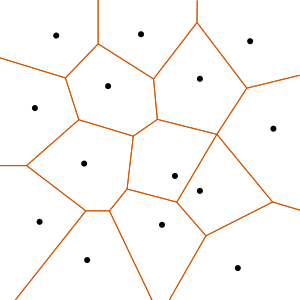
\includegraphics[keepaspectratio,scale=0.6]{images/Voronoi-Diagramm}
	\caption{Beispiel eines Voronoi-Diagramm}
	\label{graph-voronoi}
\end{figure}
\newpage
Das Problem dabei ist das durch Ausreißer, Rauschen oder Fehleingaben sich eine Überanpassung einstellen kann. In unserem Fall könnte eine sehr gute oder schlechte Bewertung die neue Bewertung stark beeinflussen und eine Firma ins Abseits schieben. Der k-Nearest-Neighbour-Algorithmus ist eine Verbesserung, die nicht nur den nächsten Nachbarn sondern die k nächsten Nachbarn betrachtet. Für k=3 also die 3 nächsten Nachbarn.

Der beschriebene Algorithmus (inkl. Verbesserung) zählt zu den \textit{lazy learning} (faules Lernen) Verfahren, weil bei der Berechnung immer alle Trainingsdaten benutzt werden. Dies ist bei kleinen Datenmengen jedoch unkritisch.

% % Raus weil wir das nicht machen, und wir auch nicht wirklich den nn-algo nutzen!! (karl)

%Aus diesem Grund verwenden wir den k-Nearest-Neighbour-Algorithmus zur Klassifikation. Dieser betrachtet nicht nur einen Punkt aus der Menge  sondern die seine K Nachbarn mit minimalem Abstand. Problematisch wird dabei aber das weiter entfernte Punkte meist die direkten Nachbarn dominieren. Um dies zu verhindern, werden die k-Nachbarn gewichtet. Die Punkte werden nun mit dem Gewicht
%\begin{equation}
%\omega_i = {1 \over d(x,x_{i})^2} 	\label{eq:AbstandkNN}
%\end{equation}
%das quadratisch mit dem Abstand abnimmt, gewichtet.








